\chapter{Contribution}

\section{Introduction}
\label{sec:contribution-introduction}

In this chapter, we present the core contributions of our work on automated brain tumor detection in MRIs. Building upon the BraTS dataset \cite{Menze2015}, our pipeline integrates a deep learning–based segmentation module with a classical machine learning classifier and culminates in a user‐friendly demo application.

% The remainder of this chapter is organized as follows. In Section~\ref{sec:contribution-dataset}, we introduce the dataset and preprocessing steps. Section~\ref{sec:contribution-segmentation} details the U-Net segmentation module, including architecture and training protocol. Section~\ref{sec:contribution-classification} covers the feature engineering and SVM classification. Section~\ref{sec:contribution-demo} presents the design and functionality of our demo application. We conclude with a discussion of key findings and future directions.

\section{Proposed Framework Overview}
\label{sec:contribution-framework}
In this section, we look at our proposed fremework from a systematic perspective. The framework is designed to perform end-to-end brain tumor segmentation and classification. We will discuss the design of the final pipeline and the training workflow to achieve the desired results.

\subsection{End-to-End Inference Pipeline}
The purpose of our project is to have an end-to-end inference pipeline accepts a raw MR image as input, applies preprocessing steps, performs segmentation of the tumor region using the trained U-Net model, classifies the tumor grade via the SVM classifier, and finally outputs the original image overlaid with the segmentation mask along with the predicted grade as shown in Figure~\ref{fig:pipeline}.
\begin{figure}[H]
  \centering
  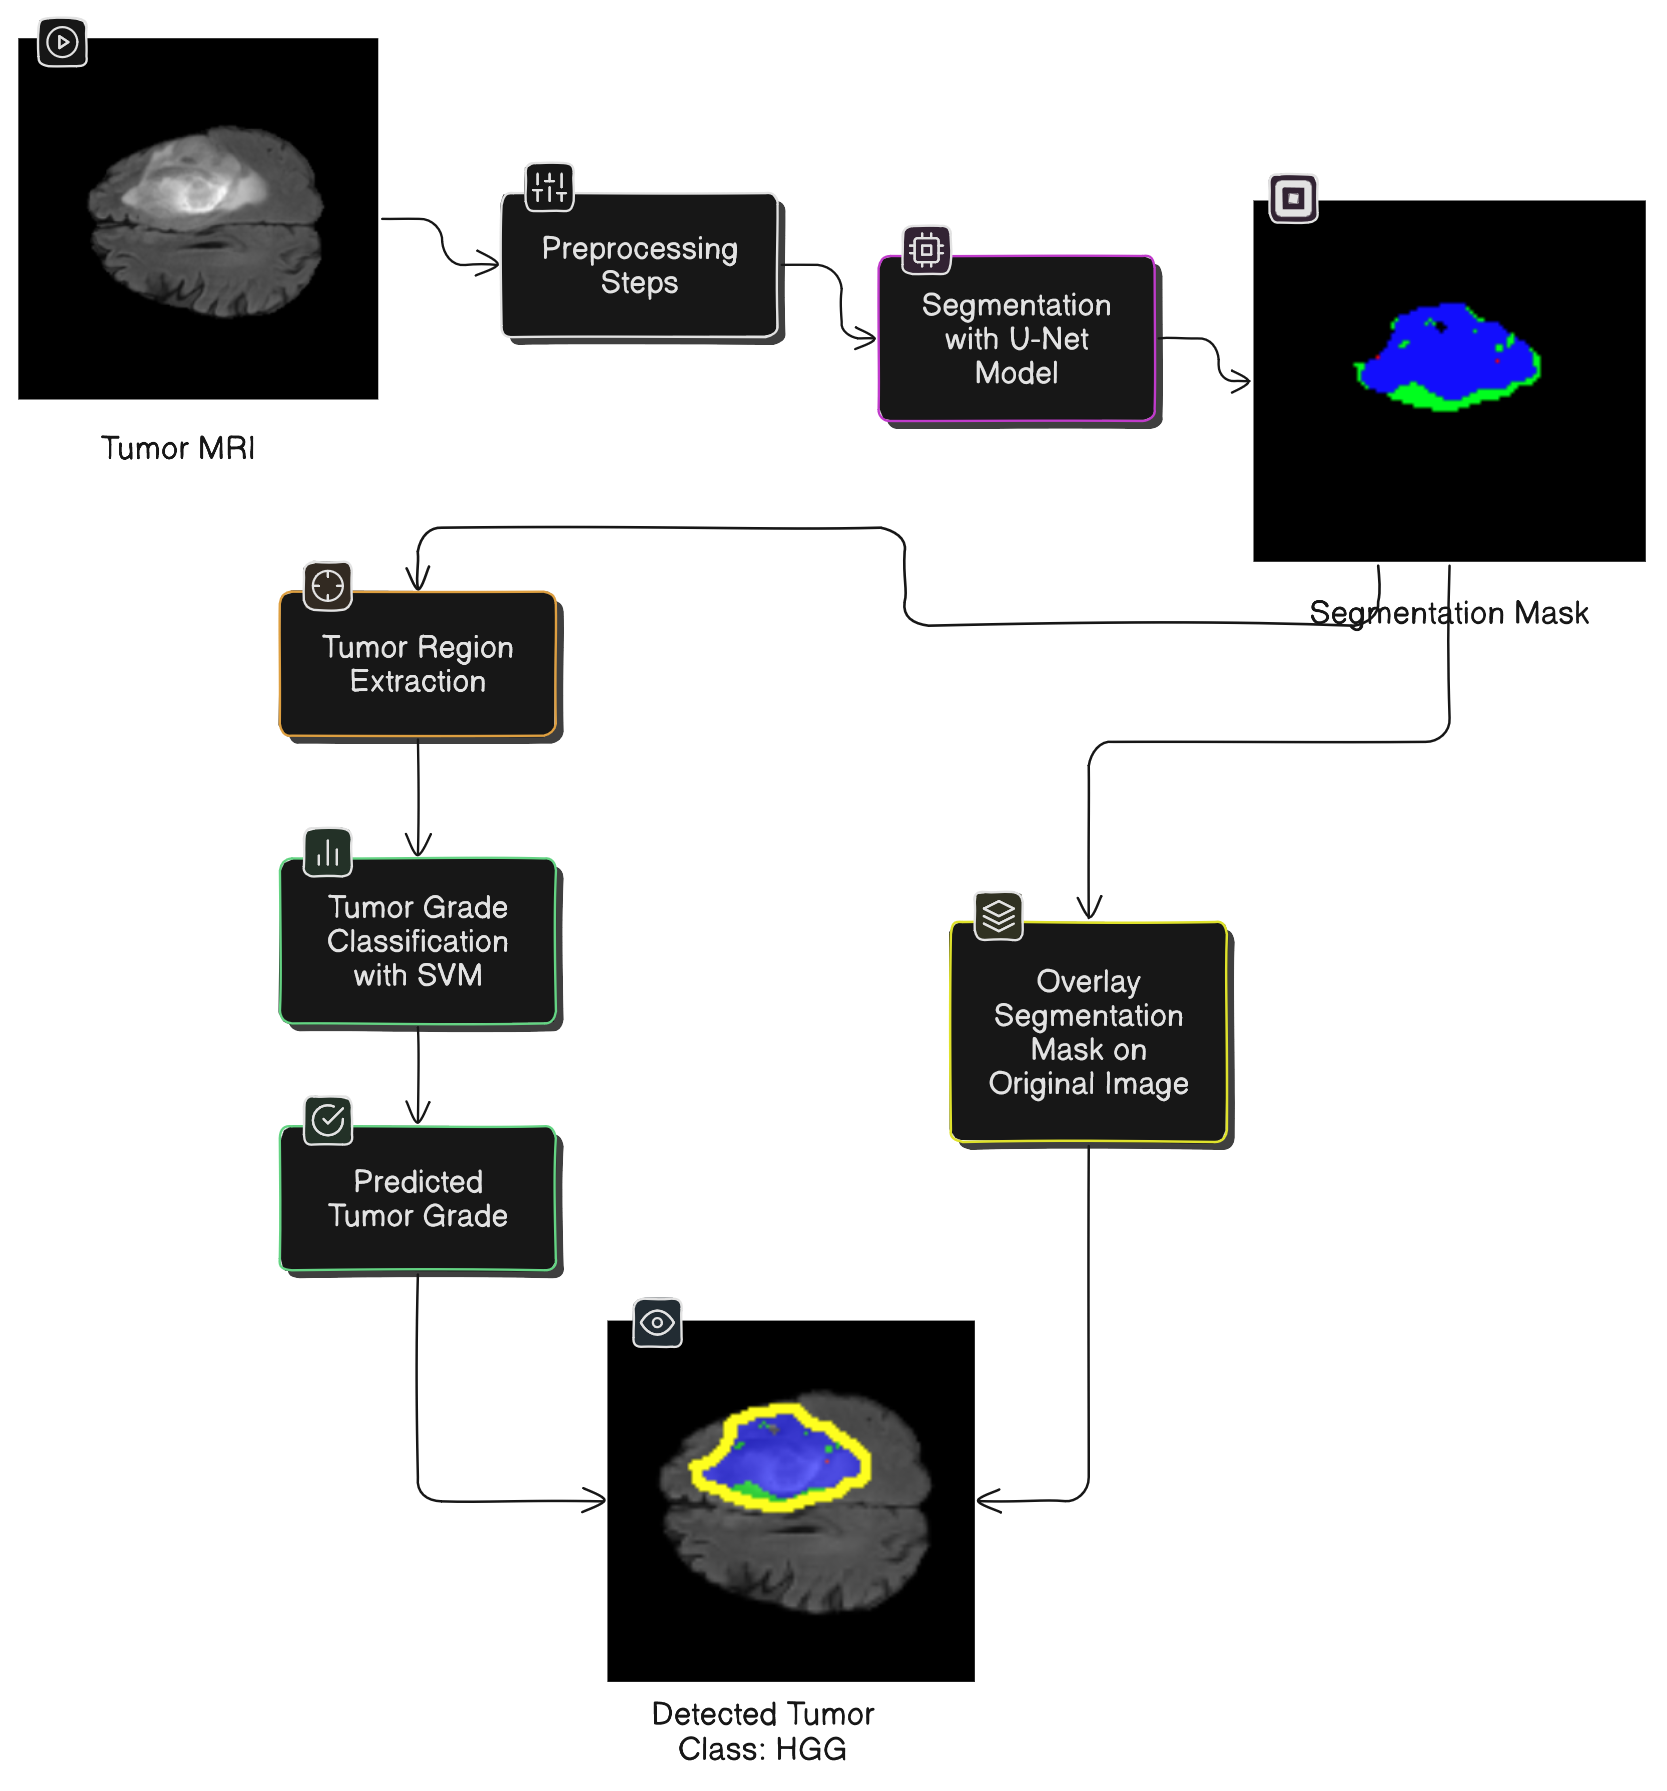
\includegraphics[width=0.8\textwidth]{Images/Chapter3/pipeline.png}
  \caption{Overview of the end-to-end inference pipeline.}
  \label{fig:pipeline}
\end{figure}
The selection of U-Net for tumor segmentation and Support Vector Machine (SVM) for tumor grade classification in our end-to-end inference pipeline is grounded in their proven efficacy in medical image analysis, particularly in brain tumor applications.

\subsubsection{U-Net for Tumor Segmentation}
U-Net is a convolutional neural network architecture specifically designed for biomedical image segmentation. Its encoder-decoder structure with skip connections allows for precise localization and context capture, making it highly effective for segmenting complex structures like brain tumors. Studies have demonstrated that U-Net and its variants achieve high accuracy in delineating tumor boundaries in MRI images, even with limited training data \cite{dong2017automatic, walsh2022using}.

Introduced by Ronneberger et al. in 2015, U-Net features a symmetric encoder-decoder structure: the contracting path (encoder) captures image context through successive convolution and pooling operations, while the expansive path (decoder) enables precise localization via upsampling and concatenation with high-resolution features from the encoder. This architecture allows U-Net to achieve accurate segmentation even with limited annotated data by leveraging extensive data augmentation. U-Net has demonstrated superior performance in various biomedical segmentation challenges, notably outperforming previous methods in tasks such as neuronal structure segmentation in electron microscopy images and cell tracking in light microscopy \cite{ronneberger2015u}.
\begin{figure}[H]
  \centering
  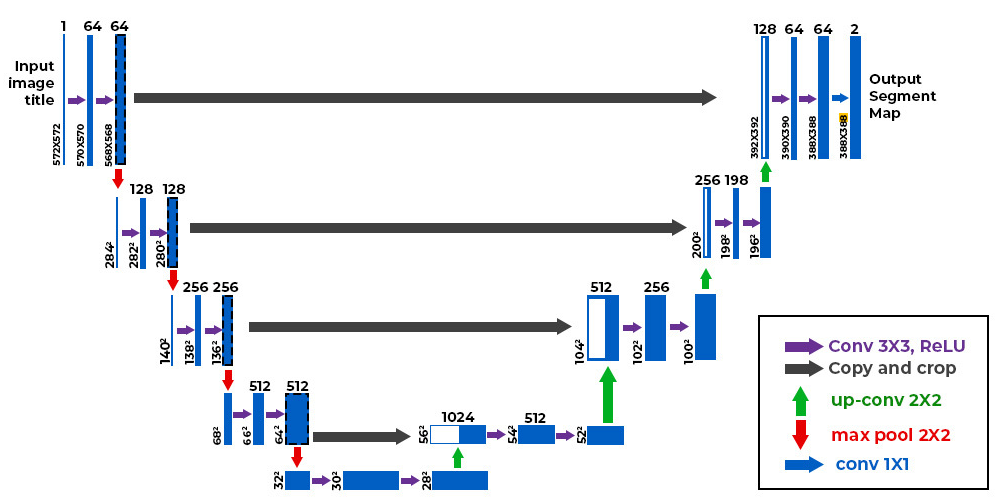
\includegraphics[width=0.8\textwidth]{Images/Chapter1/unet.png}
  \caption{U-Net Architecture Illustrating the Encoding and Decoding Arms with Skip Connections. \cite{ronneberger2015u}}
  \label{fig:unet}
\end{figure}

\paragraph*{Key Components of a U-Net Architecture}

\begin{itemize}
  \item \textbf{Contracting Path (Encoder):} \\
        This path is responsible for extracting contextual features from the input image. It consists of repeated blocks of two $3\times3$ convolutional layers (with ReLU activation), followed by a $2\times2$ max pooling operation for downsampling. With each downsampling step, the number of feature channels is doubled, allowing the network to capture increasingly abstract representations of the input.

  \item \textbf{Bottleneck:} \\
        Located at the deepest part of the network, the bottleneck consists of convolutional layers without pooling. It serves as the bridge between the encoder and decoder, capturing the most condensed and abstract features of the input.

  \item \textbf{Expansive Path (Decoder):} \\
        This path reconstructs the spatial resolution of the feature maps and enables precise localization. Each step in the decoder involves upsampling the feature map (often via transposed convolution or up-convolution), concatenating it with the corresponding feature map from the encoder (skip connection), and then applying two $3\times3$ convolutions (with ReLU activation). The number of feature channels is halved at each upsampling step.

  \item \textbf{Skip Connections:} \\
        At each level, feature maps from the encoder are concatenated with the upsampled feature maps in the decoder. These skip connections help retain high-resolution spatial information that might otherwise be lost during downsampling, improving the accuracy of segmentation boundaries.

  \item \textbf{Final Output Layer:} \\
        The last layer is typically a $1\times1$ convolution that maps each feature vector to the desired number of output classes, producing a pixel-wise classification map for segmentation tasks.
\end{itemize}

\subsubsection{SVM for Tumor Grade Classification}
SVM is a supervised machine learning algorithm known for its robustness in classification tasks, especially with high-dimensional data. In the context of brain tumor classification, SVM has been successfully employed to differentiate between tumor grades based on features extracted from MRI images. Its ability to handle non-linear relationships through kernel functions makes it suitable for capturing the subtle differences between low-grade and high-grade tumors \cite{turk2022machine, barker2016automated}.

The theoretical foundation of SVMs is based on the Structural Risk Minimization principle, which aims to minimize an upper bound on the generalization error, offering advantages over traditional Empirical Risk Minimization approaches. Originally developed by Vapnik and colleagues in the 1990s, SVMs have become popular due to their strong empirical performance and robustness to overfitting, especially in high-dimensional spaces \cite{Gunn1998SupportVM}.
\begin{figure}[H]
  \centering
  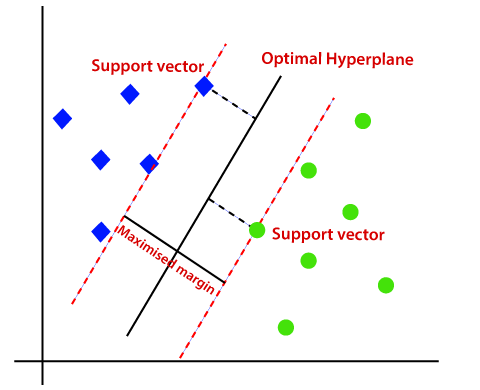
\includegraphics[width=0.5\textwidth]{Images/Chapter1/svm.png}
  \caption{Support Vector Machine (SVM) Decision Boundary Visualization}
  \label{fig:svm}
\end{figure}
The fundamental formula defining the decision boundary of a Support Vector Machine (SVM) is a hyperplane expressed as:
\begin{equation}
  \mathbf{w}^\top \mathbf{x} + b = 0
\end{equation}
where $\mathbf{w}$ is the weight vector normal to the hyperplane, $\mathbf{x}$ is the input feature vector, and $b$ is the bias term.

For binary classification with labels $y_i \in \{+1, -1\}$, the SVM enforces the following constraints on each training point $(\mathbf{x}_i, y_i)$:
\begin{equation}
  y_i \bigl(\mathbf{w}^\top \mathbf{x}_i + b\bigr) \;\ge\; 1,
  \quad \forall\,i.
\end{equation}

The margin width (the distance between the closest points of each class to the hyperplane) is given by $\tfrac{2}{\|\mathbf{w}\|_2}$.  Maximizing this margin is therefore equivalent to minimizing $\|\mathbf{w}\|_2$, leading to the following convex optimization problem:

\begin{align}
  \min_{\mathbf{w},\,b} \quad & \frac{1}{2} \|\mathbf{w}\|_2^2,                             \\
  \text{subject to} \quad     & y_i \bigl(\mathbf{w}^\top \mathbf{x}_i + b\bigr) \;\ge\; 1,
  \quad \forall\,i.
\end{align}
\subsection{Models Training Workflow}
In order to achieve the previous objectives, we followed a step-by-step approach. As shown in Figure~\ref{fig:training}, The training workflow begins with the BraTS dataset. After preprocessing and augmentation, the data is split into training, validation, and test sets. We then train the U-Net segmentation model  in the other hand (separately) we train SVM classifier training, yielding two standalone models for inference that can be combined to form a hybrid model.

\begin{figure}[H]
  \centering
  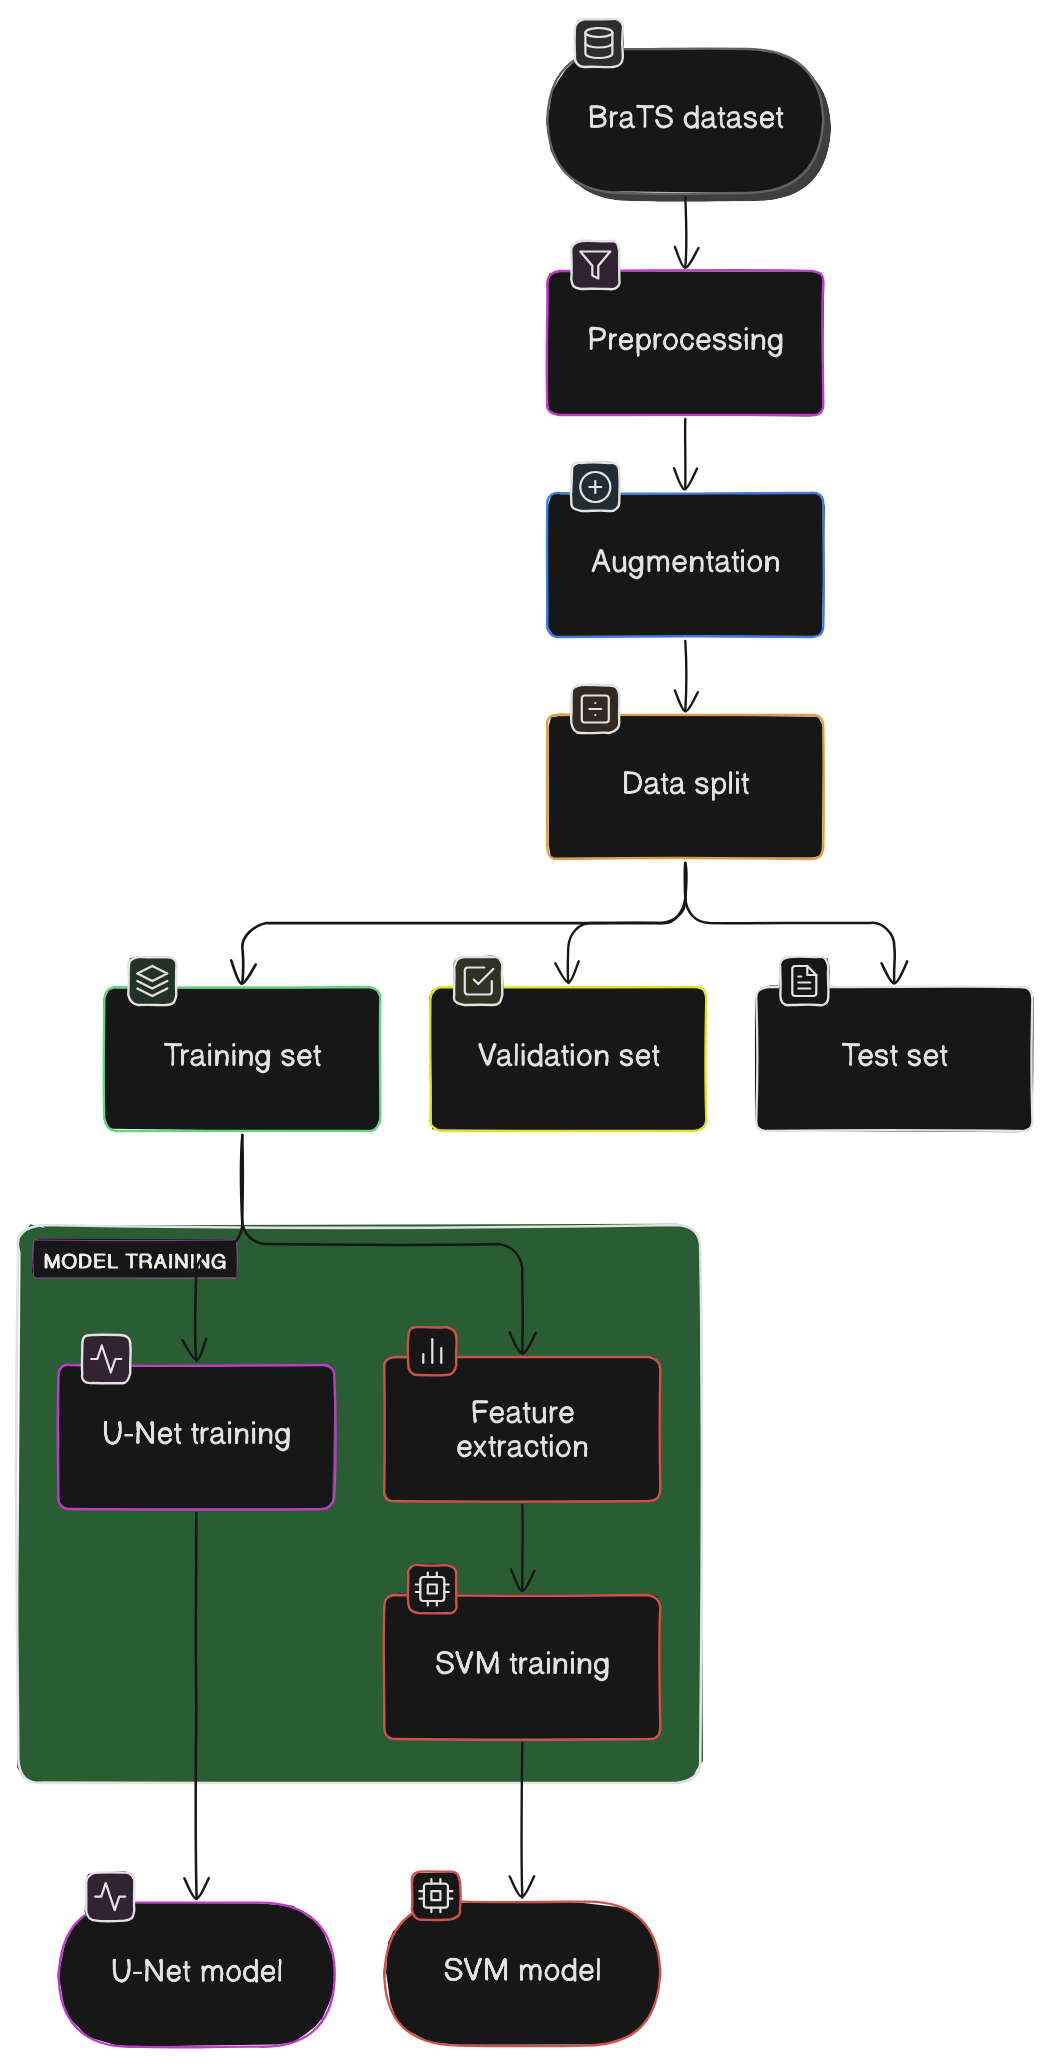
\includegraphics[width=0.6\textwidth]{Images/Chapter3/training.png}
  \caption{Overview of the training workflow.}
  \label{fig:training}
\end{figure}

\section{Dataset and Preprocessing}
\label{sec:contribution-dataset}
In order to train our hybrid model we used the Brain Tumor Segmentation (BraTS) 2020 dataset, which is a collection of multimodal Magnetic Resonance Imaging (MRI) scans used for the segmentation of brain tumors.

\subsection{BraTS Dataset Description}
The dataset includes MRI scans (Figure~\ref{fig:modalities}) from glioma patients, providing four different MRI modalities per patient:
\begin{enumerate}
  \item \textbf{Native (T1)}: Reveals detailed anatomical structures and tissue composition, aiding in the identification of tumors, cysts, and other abnormalities.
  \item \textbf{Post-contrast T1-weighted (T1ce)}: Enhances tumor visibility using a gadolinium-based contrast agent, which accentuates abnormal vascularity and lesion boundaries.
  \item \textbf{T2-weighted (T2)}: Highlights fluid content within brain tissues, which is useful for detecting edema but can sometimes obscure lesions.
  \item \textbf{T2-FLAIR (Fluid Attenuated Inversion Recovery)}: Suppresses the high signal from fluids (e.g., cerebrospinal fluid), making lesions in the white matter more conspicuous.
\end{enumerate}
\begin{figure}[H]
  \centering
  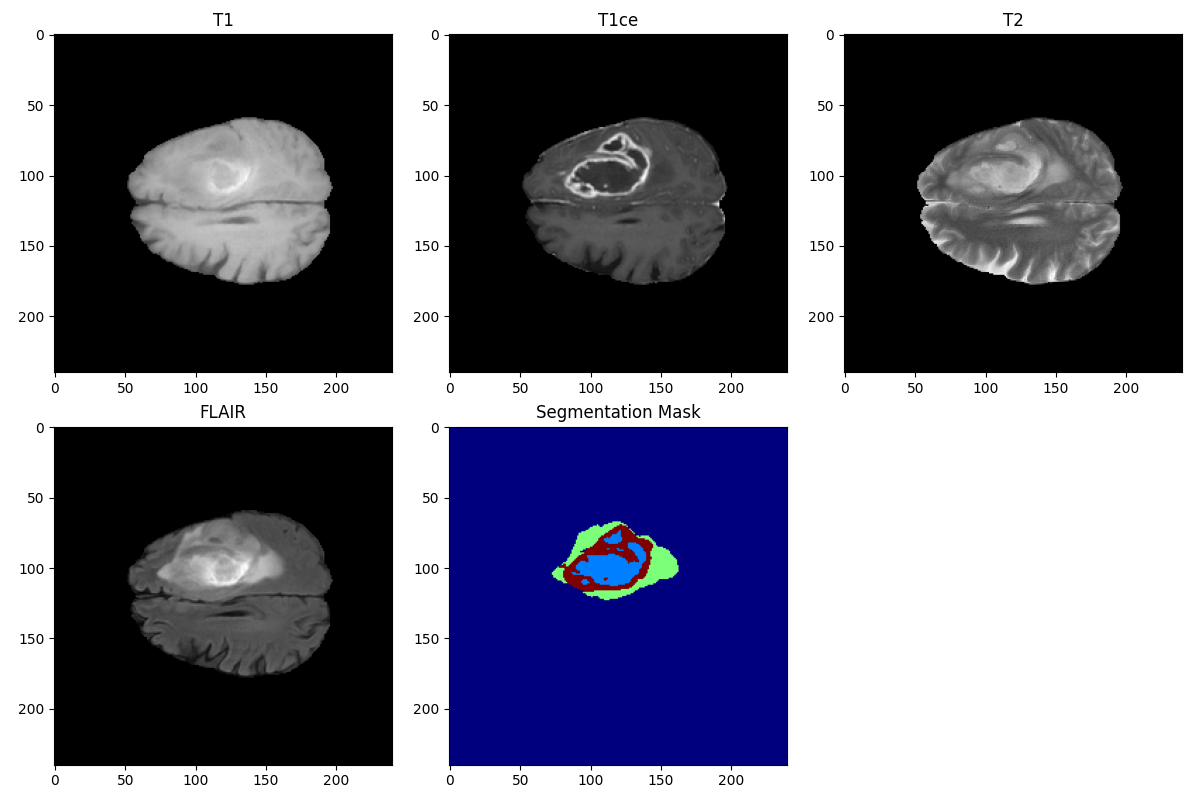
\includegraphics[width=0.8\textwidth]{Images/Chapter3/modalities.png}
  \caption{Brats modalities: T1, T1ce, T2, and T2-FLAIR.}
  \label{fig:modalities}
\end{figure}

These scans (Figure~\ref{fig:modalities}) come with expert-annotated segmentation masks that delineate the tumor into various sub-regions, such as the necrotic and non-enhancing tumor core, the peritumoral edema, and the enhancing tumor. Research has demonstrated that accurate segmentation is linked to improved prognostic assessments and treatment outcomes.

\begin{itemize}
  \item \textbf{Class 0 (Not Tumor):} This class represents normal brain tissue or background, where no tumor tissue is present.
  \item \textbf{Class 1 (Non-Enhancing Tumor):} This class corresponds to the necrotic or non-enhancing core regions of the tumor. These areas typically lack contrast enhancement and may include dead or less active tumor tissue.
  \item \textbf{Class 2 (Edema):} This class identifies regions of peritumoral edema, which is the swelling around the tumor caused by fluid accumulation. Edema is important for understanding the extent of the tumor’s impact on surrounding brain tissue.
  \item \textbf{Class 4 (Enhancing Tumor):} This class captures the actively enhancing parts of the tumor, visible after the administration of a contrast agent. These regions often indicate aggressive tumor tissue with increased blood flow and permeability.
\end{itemize}

To visually interpret these segmentations, we map the categorical labels to a custom colormap. In our example (Figure~\ref{fig:tclass}), we use four distinct colors to represent:

\begin{figure}[H]
  \centering
  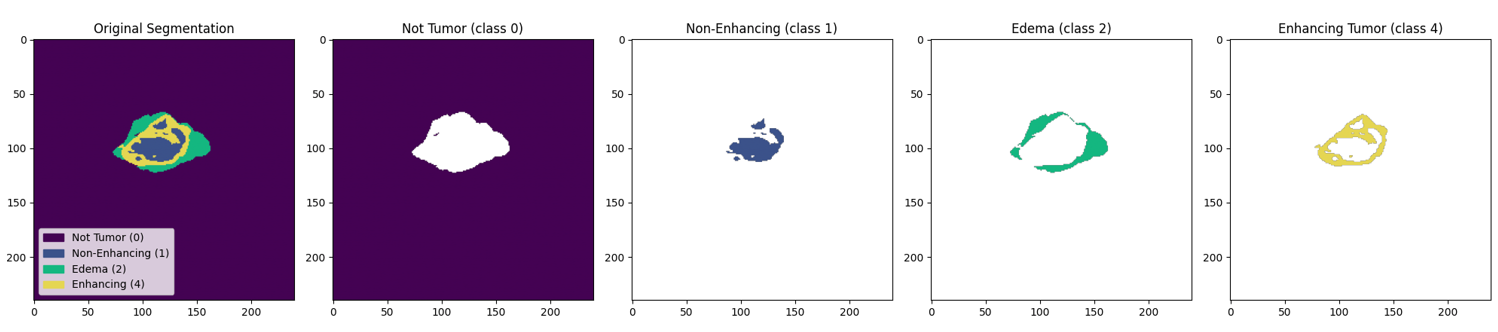
\includegraphics[width=1.1\textwidth]{Images/Chapter3/tclass.png}
  \caption{Segmentation of Tumor classes.}
  \label{fig:tclass}
\end{figure}

\subsection{Dataset Splitting}
To train and evaluate our model effectively, we need to partition our dataset into three subsets:
\begin{itemize}
  \item \textbf{Training Set (70\%):} Used to learn the model parameters.
  \item \textbf{Validation Set (approximately 20\%):} Used for tuning hyperparameters and preventing overfitting.
  \item \textbf{Test Set (10\%):} Used for assessing the final model’s performance on unseen data.
\end{itemize}
This split can be done randomly or in a stratified manner (to preserve the class distribution), which is especially useful when dealing with imbalanced datasets. Properly splitting the dataset is crucial for building a robust model that generalizes well to new data.
\begin{figure}[H]
  \centering
  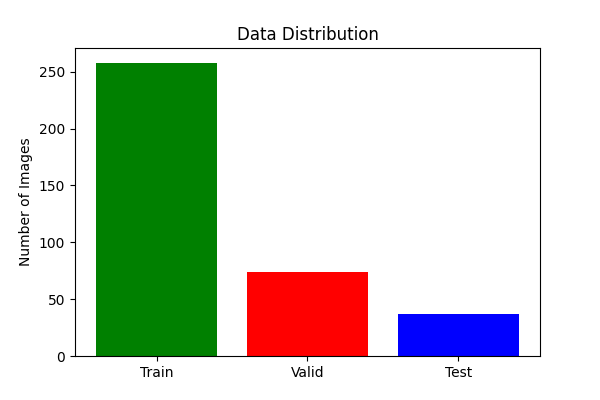
\includegraphics[width=0.8\textwidth]{Images/Chapter3/data_distribution.png}
  \caption{Dataset splitting: training, validation, and test sets.}
  \label{fig:data_distribution}
\end{figure}


\subsection{Data Preprocessing}
\label{sec:contribution-preprocessing}

Before feeding MR volumes into our models, we apply a series of standardized preprocessing steps to ensure consistency and improve model robustness. Our pipeline operates on 2D axial slices extracted from 3D volumes, as follows:

\begin{enumerate}
  \item \textbf{Slice Extraction.}
        For each patient volume, we select 100 consecutive axial slices starting at index 22. This avoids initial and final slices that contain little anatomical information.

  \item \textbf{Resizing.}
        \begin{itemize}
          \item \emph{Image Slices:} Each extracted slice is resized to \texttt{128$\times$128} pixels to match the U-Net input dimensions.
          \item \emph{Segmentation Masks:} Corresponding ground-truth masks are first resized to \texttt{240$\times$240} (to preserve label fidelity) and later downsampled alongside images during one-hot encoding.
        \end{itemize}

  \item \textbf{Intensity Normalization.}
        All pixel intensities in a slice are divided by the global maximum value of that volume, scaling inputs to the \([0,1]\) range. This step harmonizes contrast across patients and modalities.

  \item \textbf{Augmentation.}
        To increase effective training diversity, random geometric transformations are applied during batch generation:
        \begin{itemize}
          \item Horizontal and vertical flips (each with 50\% probability).
          \item Rotations by multiples of 90° (randomly chosen among 0°, 90°, 180°, 270°).
        \end{itemize}
\end{enumerate}


\section{Evaluation Metrics}
\label{sec:evaluation-metrics}

To quantify the performance of our segmentation and classification models, we use a suite of metrics that assess accuracy, robustness, and specificity:

\begin{itemize}
  \item \textbf{Accuracy}
        \[
          \text{Accuracy} \;=\; \frac{\text{TP} + \text{TN}}{\text{TP} + \text{TN} + \text{FP} + \text{FN}}
        \]
        \begin{itemize}
          \item \emph{Segmentation:} Proportion of correctly classified pixels (tumor vs.\ non‐tumor).
          \item \emph{Classification:} Proportion of correctly classified patients (LGG vs.\ HGG).
        \end{itemize}

  \item \textbf{Precision} (Positive Predictive Value)
        \[
          \text{Precision} \;=\; \frac{\text{TP}}{\text{TP} + \text{FP}}
        \]
        \begin{itemize}
          \item \emph{Segmentation:} Fraction of predicted tumor pixels that are actually tumor.
          \item \emph{Classification:} Fraction of patients predicted as HGG who truly have HGG.
        \end{itemize}

  \item \textbf{Recall} (Sensitivity or True Positive Rate)
        \[
          \text{Recall} \;=\; \frac{\text{TP}}{\text{TP} + \text{FN}}
        \]
        \begin{itemize}
          \item \emph{Segmentation:} Fraction of actual tumor pixels correctly identified.
          \item \emph{Classification:} Fraction of actual HGG patients correctly identified.
        \end{itemize}

  \item \textbf{Specificity} (True Negative Rate)
        \[
          \text{Specificity} \;=\; \frac{\text{TN}}{\text{TN} + \text{FP}}
        \]
        \begin{itemize}
          \item \emph{Segmentation:} Fraction of non‐tumor pixels correctly classified as non‐tumor.
          \item \emph{Classification:} Fraction of actual LGG patients correctly identified as LGG.
        \end{itemize}

  \item \textbf{F1‐Score}
        \[
          \text{F1} \;=\; \frac{2\,\text{TP}}{2\,\text{TP} + \text{FP} + \text{FN}}
        \]
        \begin{itemize}
          \item \emph{Classification:} Harmonic mean of precision and recall for each class, then averaged.
        \end{itemize}

  \item \textbf{Intersection over Union (IoU)}
        Also called Jaccard index:
        \[
          \text{IoU} \;=\; \frac{\text{TP}}{\text{TP} + \text{FP} + \text{FN}}
        \]
        \begin{itemize}
          \item \emph{Segmentation:} Overlap between predicted and ground‐truth tumor masks, averaged over classes (mIoU).
        \end{itemize}

  \item \textbf{Dice Coefficient} (Segmentation F1)
        \[
          \text{Dice} \;=\; \frac{2\,\text{TP}}{2\,\text{TP} + \text{FP} + \text{FN}}
        \]
        \begin{itemize}
          \item \emph{Segmentation:} Emphasizes overlap; computed overall and per‐class (necrotic, edema, enhancing).
        \end{itemize}

  \item \textbf{Confusion Matrix}
        A contingency table of true vs.\ predicted labels:
        \[
          \begin{array}{c|cc}
                                   & \text{Predicted Positive} & \text{Predicted Negative} \\ \hline
            \text{Actual Positive} & \text{TP}                 & \text{FN}                 \\
            \text{Actual Negative} & \text{FP}                 & \text{TN}                 \\
          \end{array}
        \]
        \begin{itemize}
          \item \emph{Classification:} Provides counts of TP, FP, FN, TN for LGG/HGG.
        \end{itemize}

  \item \textbf{ROC AUC} (Area Under the Receiver Operating Characteristic Curve)
        \[
          \text{AUC} \;=\; \frac{1}{2} \sum_{i=1}^{n} (\text{TPR}_{i} + \text{TPR}_{i-1}) \times (\text{FPR}_{i} - \text{FPR}_{i-1})
        \]

        \begin{itemize}
          \item \emph{Classification:} Measures the trade‐off between sensitivity and specificity across thresholds.
        \end{itemize}
        \paragraph{knowing that:}
        \begin{itemize}
          \item \(\text{TP}\) = number of true positive cases (correctly predicted positive).
          \item \(\text{TN}\) = number of true negative cases (correctly predicted negative).
          \item \(\text{FP}\) = number of false positive cases (incorrectly predicted positive).
          \item \(\text{FN}\) = number of false negative cases (incorrectly predicted negative).
          \item \(\text{TPR}\) = true positive rate (recall): \(\text{TPR} = \frac{\text{TP}}{\text{TP} + \text{FN}}\).
          \item \(\text{FPR}\) = false positive rate: \(\text{FPR} = \frac{\text{FP}}{\text{FP} + \text{TN}}\).
          \item \(\text{TNR}\) = true negative rate (specificity): \(\text{TNR} = \frac{\text{TN}}{\text{TN} + \text{FP}}\).
          \item \(\text{FNR}\) = false negative rate: \(\text{FNR} = \frac{\text{FN}}{\text{FN} + \text{TP}}\).
        \end{itemize}

\end{itemize}




\section{Results and Discussion}




\subsection{Segmentation Results}
\label{sec:segmentation-results}
In this section, we present the results of our U-Net segmentation model on the BraTS2020 dataset. The model was trained for 50 epochs with a batch size of 16, we will discuss the end results of the training and validation process, including loss and accuracy metrics.

\subsubsection{Accuracy}
The model achieved an impressive pixel-level accuracy of 99.3\%, indicating that the vast majority of pixels were correctly classified. This high accuracy is particularly important in medical imaging, where even small errors can have significant implications. The overall results shown in Figure~\ref{fig:unet-acc} provide a clear picture of the training and validation accuracy over the course of the training process.
\begin{figure}[ht]
  \centering
  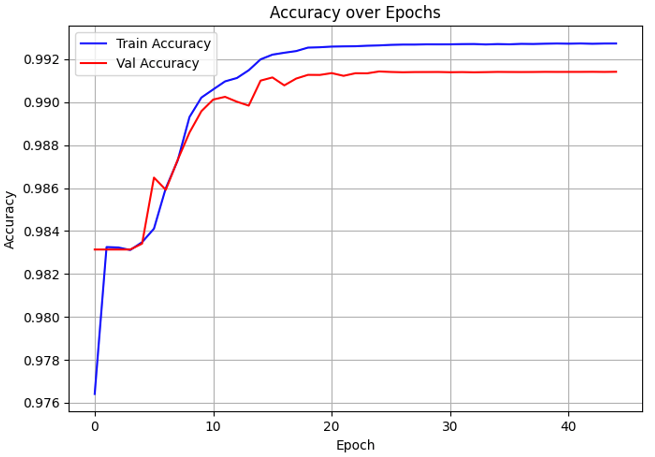
\includegraphics[width=0.7\textwidth]{Images/Chapter3/unet_acc.png}
  \caption{Training and Validation Accuracy over Epochs for the U-Net Segmentation Model}
  \label{fig:unet-acc}
\end{figure}
\\
\\
\subsubsection{Loss}
The loss function used during training was the categorical cross-entropy loss, which measures the dissimilarity between the predicted and true distributions. The model converged to a low loss of 0.0231, indicating that the predictions were closely aligned with the ground truth. The loss curve shown in Figure~\ref{fig:unet-loss} provides a clear picture of the training and validation loss over the course of the training process.

\begin{figure}[h]
  \centering
  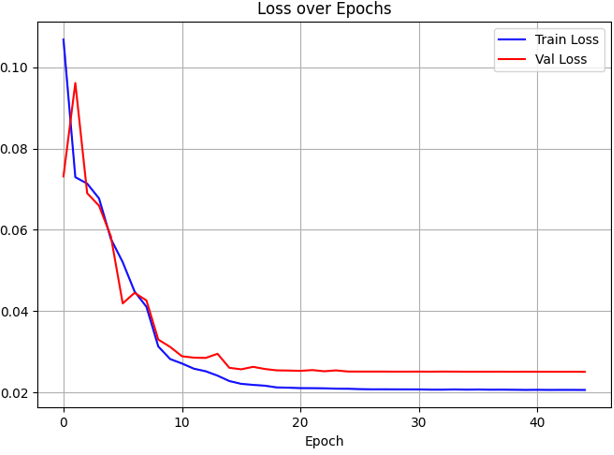
\includegraphics[width=0.7\textwidth]{Images/Chapter3/unet_loss.png}
  \caption{Training and Validation Loss over Epochs for the U-Net Segmentation Model}
  \label{fig:unet-loss}
\end{figure}

\subsubsection{Dice Coefficient}
The Dice coefficient is a measure of overlap between the predicted and true segmentation masks. The overall Dice coefficient achieved was 58.98\%, indicating a good level of agreement between the predicted and true tumor regions. The per-class Dice coefficients were also calculated, providing insights into the model's performance on different tumor subregions. The results shown in Figure~\ref{fig:unet-dice} provide a clear picture of the training and validation Dice Coefficient over the course of the training process.
\begin{figure}[h]
  \centering
  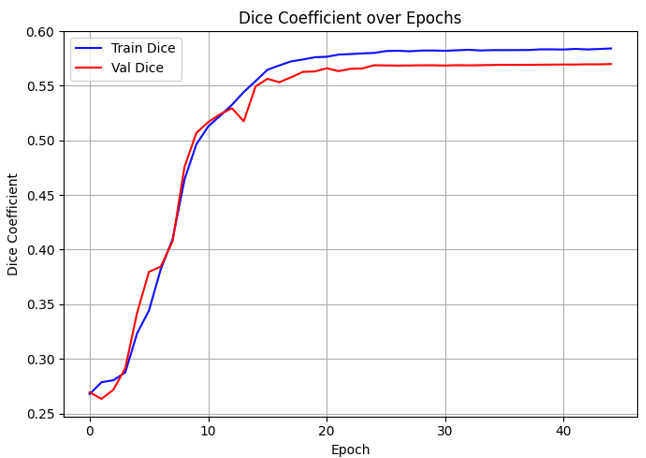
\includegraphics[width=0.7\textwidth]{Images/Chapter3/unet_dice.png}
  \caption{Training and Validation Dice Coefficient over Epochs for the U-Net Segmentation Model}
  \label{fig:unet-dice}
\end{figure}


\subsubsection{Mean IoU}
The mean Intersection over Union (IoU) was calculated to assess the model's performance across all classes. The mean IoU achieved was 74.66\%, indicating a good level of overlap between the predicted and true segmentation masks. This metric is particularly useful in medical imaging, where accurate delineation of tumor boundaries is crucial for treatment planning. The results shown in Figure~\ref{fig:unet-iou} provide a clear picture of the training and validation Mean IoU over the course of the training process.
\begin{figure}[h]
  \centering
  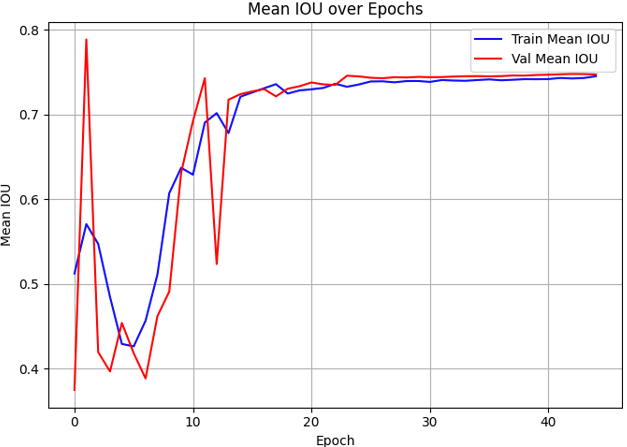
\includegraphics[width=0.7\textwidth]{Images/Chapter3/unet_iou.png}
  \caption{Training and Validation Mean IoU over Epochs for the U-Net Segmentation Model}
  \label{fig:unet-iou}
\end{figure}
\\
\\
\subsubsection{Summary}
Table~\ref{tab:segmentation-results} summarizes the quantitative performance of the U-Net segmentation model. The overall accuracy of the model is 99.30\%, which is a measure of the proportion of correctly classified pixels. The mean IoU of 74.66\% indicates a good level of overlap between the predicted and true segmentation masks across all classes. The Dice coefficient of 58.98\% is a measure of the overlap between the predicted and true tumor regions. The precision of 99.37\% indicates a low number of false positives, while the sensitivity of 99.08\% indicates a low number of false negatives. The specificity of 99.79\% indicates that the model is effective at eliminating false positives. The results shown in Figure~\ref{fig:segmentation-example} provide a clear picture of the predicted tumor segmentation masks.

\begin{table}[ht]
  \centering
  \caption{Performance Metrics for the U-Net Segmentation Model}
  \label{tab:segmentation-results}
  \begin{tabular}{l r}
    \hline
    \textbf{Metric}            & \textbf{Value} \\
    \hline
    Loss                       & 0.0231         \\
    Accuracy                   & 99.30\,\%      \\
    Mean IoU                   & 74.66\,\%      \\
    Dice Coefficient (overall) & 58.98\,\%      \\
    Precision                  & 99.37\,\%      \\
    Sensitivity                & 99.08\,\%      \\
    Specificity                & 99.79\,\%      \\
    \hline
  \end{tabular}
\end{table}

\begin{figure}[h]
  \centering
  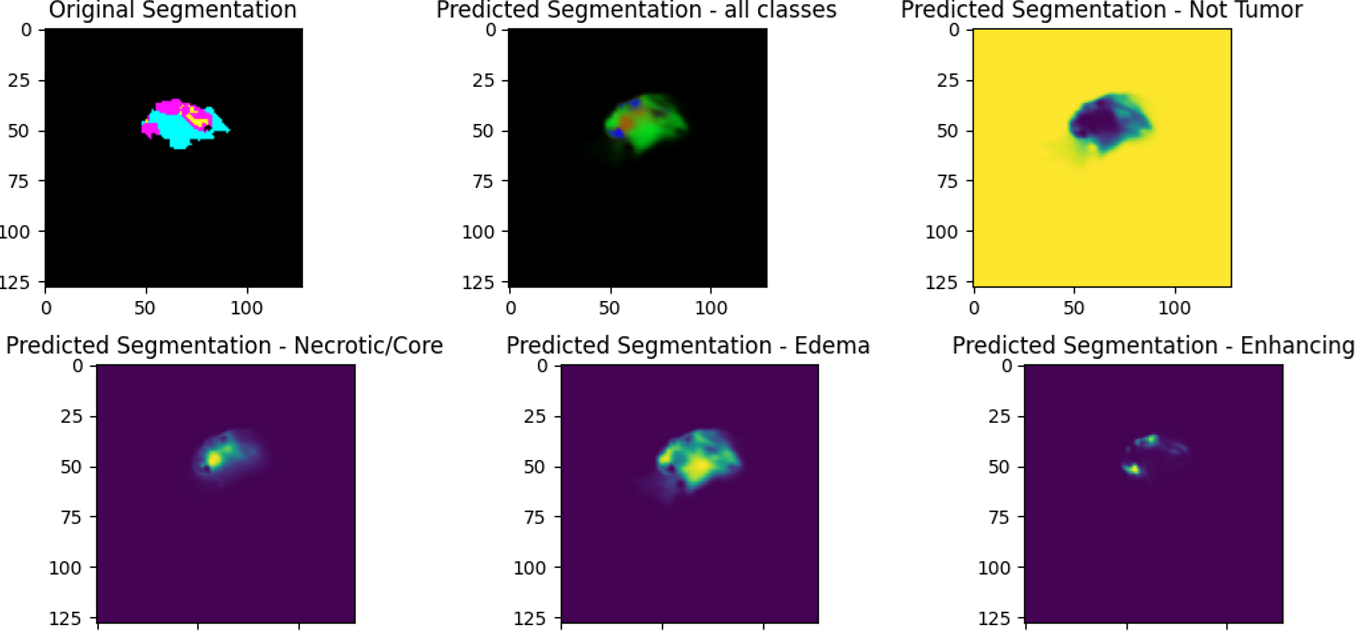
\includegraphics[width=0.9\textwidth]{Images/Chapter3/seg.png}
  \caption{Sample of a Predicted tumor segmentation masks.}
  \label{fig:segmentation-example}
\end{figure}


\subsection{Classification Results}
\label{sec:classification-results}

Table~\ref{tab:svm-report} summarizes the classification performance of the Support Vector Machine (SVM) model on the held-out test set. The model achieved an overall accuracy of 93.24\,\%, indicating strong generalization. High-grade gliomas (HGG) were classified with high precision (95\,\%) and recall (97\,\%), resulting in an F1-score of 96\,\%. In contrast, low-grade gliomas (LGG) achieved slightly lower metrics, with an F1-score of 83\,\%, reflecting a minor challenge in capturing the more subtle features associated with LGG.

The macro average shows a balanced view of precision and recall across both classes, with scores around 88–90\,\%, while the weighted average—which takes class support into account—remains consistent at 93\,\%. These results confirm the SVM model's reliability and effectiveness in brain tumor grade classification, particularly in detecting HGG, which typically has more distinct patterns and features.

\begin{table}[ht]
  \centering
  \caption{Performance Metrics of SVM Classifier on the Test Set}
  \label{tab:svm-report}
  \begin{tabular}{lcccc}
    \hline
    Class        & Precision                     & Recall & F1-Score & Support \\
    \hline
    LGG (0)      & 86\,\%                        & 80\,\% & 83\,\%   & 15      \\
    HGG (1)      & 95\,\%                        & 97\,\% & 96\,\%   & 59      \\
    \hline
    Accuracy     & \multicolumn{4}{c}{93.24\,\%}                               \\
    Macro avg    & 90\,\%                        & 88\,\% & 89\,\%   & 74      \\
    Weighted avg & 93\,\%                        & 93\,\% & 93\,\%   & 74      \\
    \hline
  \end{tabular}
\end{table}

\begin{figure}[H]
  \centering
  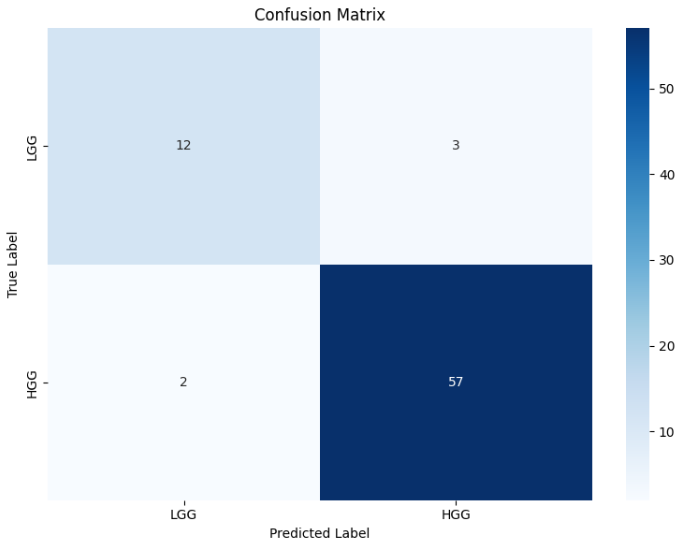
\includegraphics[width=0.6\textwidth]{Images/Chapter3/confusion.png}
  \caption{Confusion matrix for the SVM classifier.}
  \label{fig:confusion}
\end{figure}

\paragraph{Example Inference}
On a new patient (ID 083), the pipeline predicted:
\begin{itemize}
  \item \textbf{Prediction:} HGG
  \item \textbf{Probability of HGG:} 93.60\,\%
  \item \textbf{Actual Grade:} HGG (correct)
\end{itemize}

\section{Application Demo}
\label{sec:contribution-demo}

To illustrate end‐user interaction, we developed a lightweight demo application that integrates our trained U-Net and SVM models into a single GUI. The application  consists of two main pages:

\subsection{Upload Page}
\label{sec:contribution-demo-upload}

Presents an HTML form where the user can select and upload a brain tumor image (2D slice).
Upon submission, the form sends a POST request to the \texttt{/results} route.

\begin{figure}[H]
  \centering
  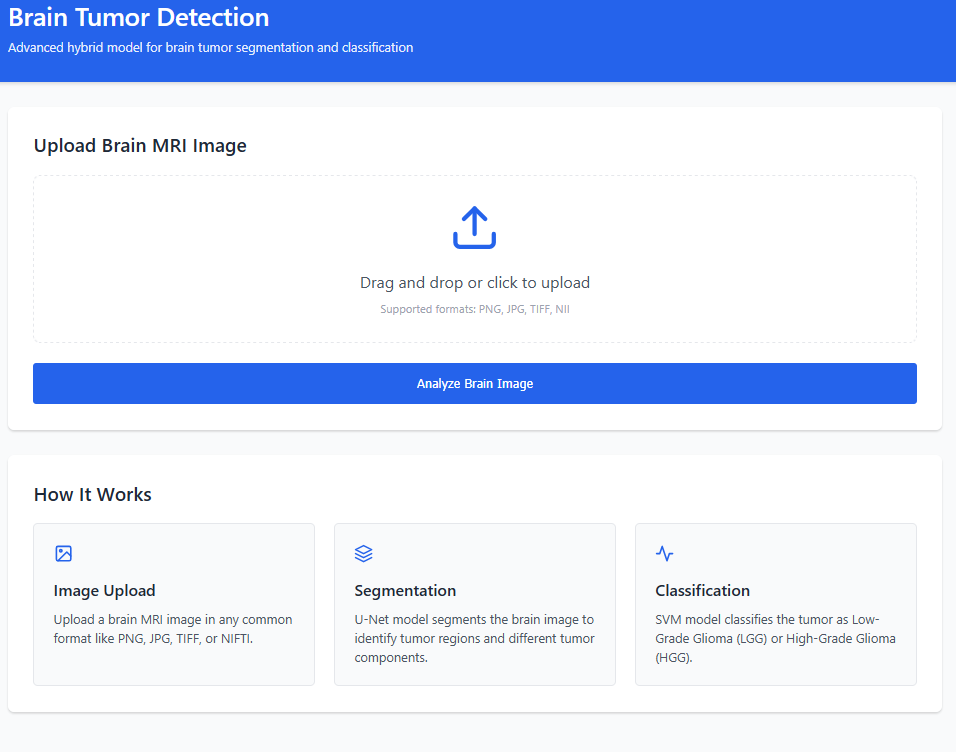
\includegraphics[width=1\textwidth]{Images/Chapter3/app_interface.png}
  \caption{Upload page of the application demo.}
  \label{fig:demo-upload}
\end{figure}

\subsection{Results Page}
\label{sec:contribution-demo-results}

Receives the uploaded image, runs the preprocessing, segmentation (U-Net), feature extraction, and classification (SVM) pipeline, and then renders:
\begin{itemize}
  \item The original input image.
  \item The segmentation mask overlaid on the input.
  \item The predicted tumor grade (LGG/HGG) with its confidence score.
\end{itemize}
\begin{figure}[H]
  \centering
  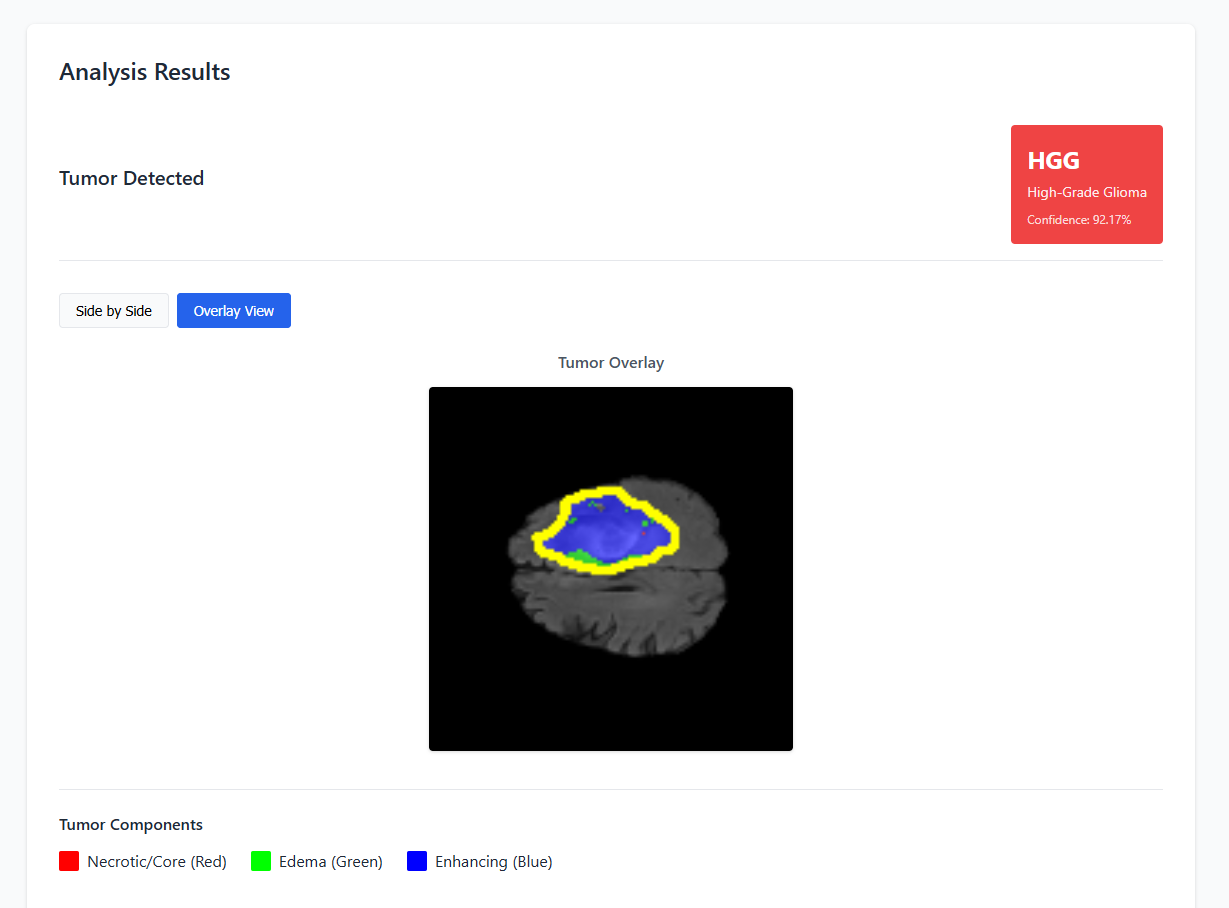
\includegraphics[width=1\textwidth]{Images/Chapter3/app_result.png}
  \caption{Results page of the application demo.}
  \label{fig:demo-results}
\end{figure}

\section{Conclusion}
\label{sec:contribution-conclusion}

In this chapter, we have presented a comprehensive methodology for automated brain tumor detection and classification using MR images. Our approach integrates a U-Net-based segmentation model with an SVM classifier, achieving high accuracy and robust performance across multiple evaluation metrics. The segmentation module demonstrated reliable delineation of tumor subregions, while the classification module effectively distinguished between high-grade and low-grade gliomas. Additionally, we showcased the practical application of our framework through a user-friendly demo application, highlighting its potential for real-world clinical use. These contributions underscore the effectiveness of combining deep learning and classical machine learning techniques in addressing complex medical imaging challenges. Future work could explore further optimization of the pipeline, incorporation of additional data modalities, and validation on larger, more diverse datasets.



